
 \section*{Introduction}

L'analyse harmonique (fréquentielle) des systèmes permet de mettre en évidence de nombreuses caractéristiques telles que la bande passante, la fréquence de coupure, la résonance, etc.
Elle sera aussi très utile pour étudier la stabilité d'un système en 2\up{nde} année.

Un système modélisé linéaire peut se caractériser dans le domaine symbolique de Laplace par sa fonction de transfert $H(p)$. Sa forme générale est :

$H(p) = \frac{{{a_m}{p^m} + ... + {a_1}p + {a_0}}}{{{b_n}{p^n} + ... + {b_1}p + {b_0}}}$ où les coefficients $a_i, i \in [0;m]$ et $b_k, k \in [0;n]$ sont réels.

La variable $p$ est un nombre complexe. Pour l'analyse fréquentielle, on pose $p=j \omega$ ($p\in \C)$. C'est le cas particulier de la transformée de Fourier. On parle alors aussi de transmittance $H(j \omega)$.

Une représentation classique de cette fonction, est le diagramme de Bode (figure \ref{Fig1}). Il fait apparaître deux quantités : le gain (dB) et la phase (\degres).

\begin{figure}[!h]
\begin{center}
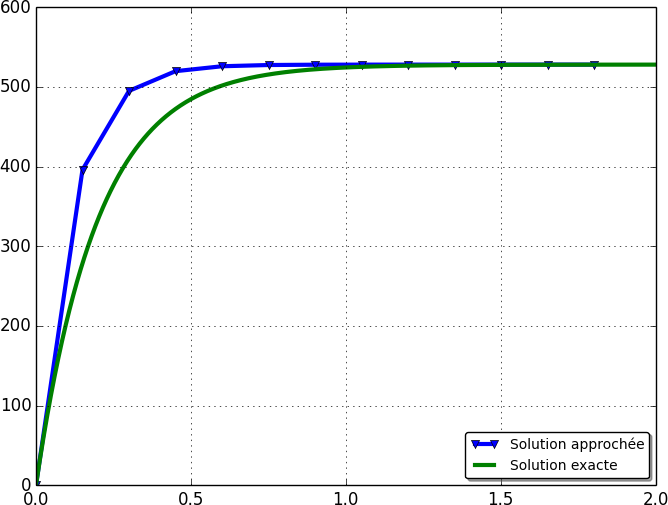
\includegraphics[scale=0.4]{figure_1.png} 
\caption{\label{Fig1} Diagrammes de Bode de systèmes du 2\up{nd} ordre}
\end{center}
\end{figure}

\begin{dBox}
\textit{L'objectif des questions qui suivent est d'extraire certaines propriétés d'un système linéaire à partir de sa fonction de transfert.}
\end{dBox}


 \section*{Diagramme de Bode}

Le tracé de la figure \ref{Fig1} a été obtenu à l'aide du script donné en annexe 1.

 
\question{} En analysant le script donné en annexe 1, donner les fonctions de transfert dont le diagramme de Bode est représenté sur la figure \ref{Fig1} ?
 

 
\question{} A une étape de l'algorithme proposé, 
\begin{enumerate}
\item combien de données contiennent les listes \texttt{w}, \texttt{gain} et \texttt{phase} ?
\item Donner le nombre de bits nécessaire au codage des flottant en double précision.
\item En admettant que chacune de ces données est de type \texttt{float} codé en double précision, quelle quantité de mémoire est nécessaire pour le stockage de ces trois listes ?
\end{enumerate}

 


 \section*{Propriétés caractéristiques du système}

\subsection*{Asymptote infinie de la courbe en gain}

Trois listes de même dimension \texttt{w}, \texttt{gain} et \texttt{phase} contiennent les données permettant le tracé.
On souhaite déterminer l'asymptote lorsque $\omega \to \infty$ de la courbe de gain de la figure 1. 

 
\question{} Proposer une instruction permettant de donner la valeur de l'asymptote lorsque $\omega \to \infty$ de la courbe de gain en dB/decade (décibels par décade).
 

\subsection*{Résonance}

Les courbes en \textbf{gain} de la figure \ref{Fig1} présentent \textbf{un maximum} appelé << pic de résonance >>. En effet, lorsque le gain est positif, c'est qu'il y a amplification du signal d'entrée.

Dans le contexte de la figure \ref{Fig1} (au maximum un seul pic de réconance), on donne ci-dessous la fonction \texttt{picResonance(w,gain,phase)} qui retourne pour une courbe un triplet de valeurs respectives la pulsation de résonance \textit{wr}, le gain maximal \textit{gr} et la phase correspondante \textit{pr} : \texttt{(wr,gr,pr)}.

%\begin{dBox}
%\lstinputlisting[language=Python,firstnumber=1,numbers=left]{Algorithmes/pic.py}
%\end{dBox}

\begin{lstlisting}
def picResonance(w,gain,phase):
    n=len(w)
    gr=gain[0]
    i=1
    while i<n and gr<=gain[i]:
        gr=gain[i]
        i+=1
    if i==1:
        return ()
    else:
        return (w[i-1],gr,phase[i-1])
\end{lstlisting}


 
\question{} Pour la fonction proposée (\texttt{picResonance(w,gain,phase)}, proposer un invariant de boucle. Dans le cas où ce pic n'existerait pas, que renvoie la fonction ? Proposer un variant de boucle et démontrer que l'algorithme renvoie bien un résultat.
 



Dans certains cas, le système peut présenter plusieurs pics de résonance (figure \ref{Fig2}).

\begin{figure}[!h]
\begin{center}
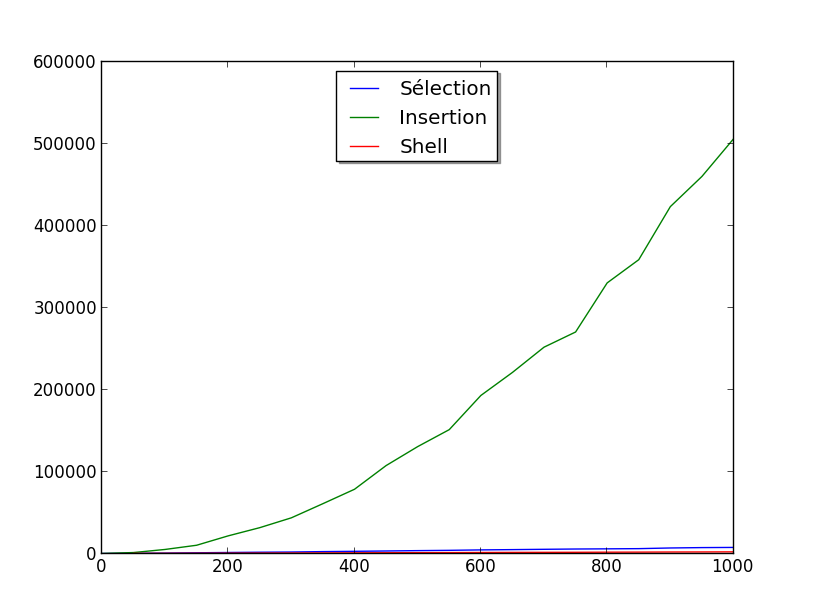
\includegraphics[scale=0.5]{figure_2.png} 
\caption{\label{Fig2} Système multi-pics}
\end{center}
\end{figure}

 
\question{} Dans le cas où le diagramme en gain serait multi-pics, écrire la fonction \\ \texttt{picsResonance(w,gain,phase)} retournant une liste \texttt{L} de triplets de valeurs respectives une pulsation de résonance \texttt{wr}, le gain \texttt{gr} et la phase correspondante \texttt{pr} : \texttt{(wr,gr,pr)}. La liste \texttt{L} peut présenter l'allure suivante : \texttt{[(wr1,gr1,pr1),(wr2,gr2,pr2),...,(wrk,grk,prk)]}. Dans le cas où il n'y aurait aucun pics, la fonction retourne une liste vide.
 


\subsection*{Bande passante}

\begin{dBox}
Pour un filtre passe-bas, la bande passante peut être définie comme la plage de pulsations $\omega \in ]0;\omega_c]$ pour lesquelles le gain est supérieur ou égal à $G_{\text{max}}-3 \text{dB}$. On peut ainsi préciser la pulsation de coupure $\omega_c$.
\end{dBox}



Dans tout ce qui suit, on se place dans le cas d'un filtre passe-bas passif ($G_{\text{dB}}(0) = 0)$ non résonant. La fonction $G_{\text{dB}}$ est monotone décroissante et l'équation $G_\text{dB}(\omega) + 3 = 0$ admet toujours une unique solution. On est par exemple dans le cas de la figure 3. Dans la bande passante, l'atténuation du signal d'entrée ne dépasse pas alors environ 30 \%.

\begin{figure}[!h]
\begin{center}
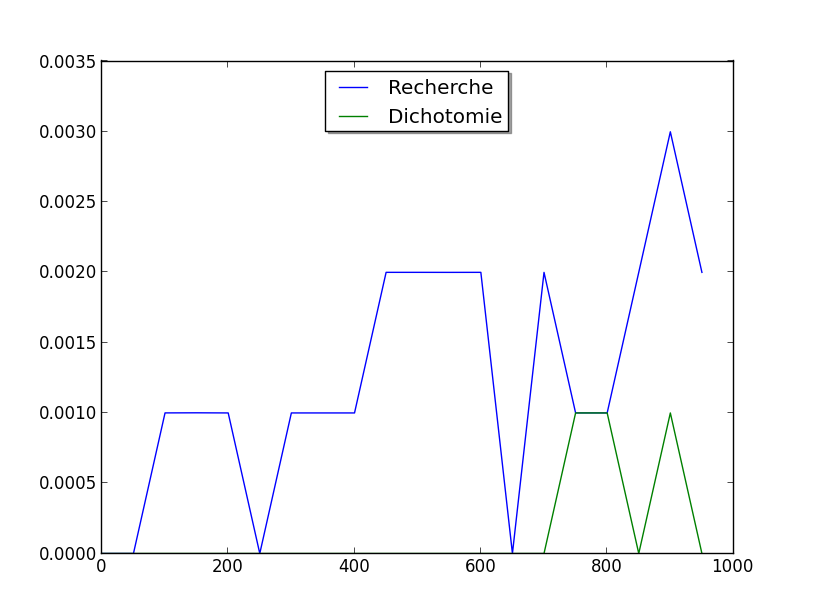
\includegraphics[scale=0.5]{figure_3.png} 
\caption{\label{Fig3} Filtre passe-bas passif non résonant}
\end{center}
\end{figure}

 
\question{} Écrire la fonction \texttt{pulsationCoupure(w,gain)} retournant la valeur de la pulsation de coupure \texttt{wc} en utilisant une méthode par balayage de la liste \texttt{gain}. On s'assurera de la terminaison de l'algorithme. Si la pulsation de coupure n'existe pas, on retourne $-1$.
 

\begin{dBox}
La méthode de dichotomie pour résoudre une équation est basée sur le théorème des valeurs intermédiaires. Soit $f : [a,b] \to \mathbb{R}$ une fonction continue, alors $f$ prend toutes les valeurs intermédiaires entre $f(a)$ et $f(b)$.
En particulier, si $f$ est telle que $f(a) \times f(b)<0$, alors il existe $\alpha \in ]a,b[$ tel que $f(\alpha) = 0$.
\end{dBox}

  
\question{} Proposer une fonction \texttt{pulsationCoupure(w,gain)} retournant la valeur de la pulsation de coupure \texttt{wc} en utilisant une méthode de dichotomie sur la liste \texttt{gain}. Si la pulsation de coupure n'existe pas, on retourne -1.
 


%  
%\question{}
%\begin{enumerate}
%\item Pour l'algorithme précédent, définir un variant de boucle et effectuer une preuve de terminaison,
%\item Définir un invariant de boucle et effectuer une preuve de correction.
%\item Quel intérêt présente la méthode de dichotomie par rapport à une méthode par balayage ?
%\end{enumerate}
% 


 \section*{Stockage des données dans un fichier texte}

On souhaite stocker le contenu des listes \texttt{w}, \texttt{gain} et \texttt{phase} dans un fichier texte \texttt{"bode.txt"}.

L'annexe 2 donne quelques fonctions python.
Par exemple, pour ouvrir un fichier en écriture, on peut écrire \texttt{f = open("bode.txt","w")}. La variable \texttt{f} est alors un objet de type fichier.

La structure attendu dans le fichier texte \texttt{"bode.txt"} est la suivante (cas de la figure 2) :

\begin{dBox}
\hspace{0.5 cm} \texttt{pulsation;gain;phase}

\texttt{0.1;0.290546581842;-0.306830090606}

\texttt{0.12;0.421009962397;-0.373102215459}

\texttt{0.14;0.577344844946;-0.442256557908}

\texttt{...}
\end{dBox}

\begin{remark}
La première ligne permet de préciser le type des données du fichier.
La suite comporte autant de lignes que de données. Les séparateurs sont des points virgules ";".
\end{remark}

 
\question{}
\begin{enumerate}
\item Quelle sera la taille approximative du fichier texte \texttt{"bode.txt"} sachant que le nombre de données est identique à celui de la question 2 et que l'on suppose les caractères sont codés en ASCII (1 caractère sur un octet) ?
\item Quel serait le gain de taille en \% si on se limitait à 3 chiffres significatifs pour chacune des valeurs numériques ?
\end{enumerate}
 

 
\question{} Écrire un script utilisant les listes \texttt{w}, \texttt{gain} et \texttt{phase}, et permettant de créer le fichier "bode.txt". A la fin de l'écriture, on assurera sa fermeture << propre >>.
 

 
\question{} Proposer une fonction \texttt{retourneListes(nomFichier)} prenant en argument une chaîne de caractère \texttt{nomFichier} et retournant les listes \texttt{w} (pulsations) et \texttt{gain} (gains). A la fin de la lecture, on assurera la fermeture << propre >> du fichier.
 

\vspace{3 cm}

\begin{center}
-- Fin de sujet --
\end{center}

\vfill


\pagebreak
\begin{center}
\huge{Annexe 1 : Diagrammes de Bode}
\end{center}
%\lstinputlisting[language=Python,firstnumber=1,numbers=left]{Algorithmes/bode.py}
\begin{lstlisting}
import numpy as np
from scipy import signal
from matplotlib import pyplot as plt

# Fonction de transfert sous la forme num(p)/den(p)
# Coefficients au numerateur
# du plus grand ordre au plus petit, exemple : 1*p^0
num = [1]
# Coefficients au denominateur
# du plus grand ordre au plus petit, exemple : 1*p^2 + 0.1*p^1 + 1*p^0
# den = [1, 0.1, 1]
 
plt.subplot(2, 1, 1)
for i in range(5):
    den = [1,0.1+i/5,1]
    #definition de la fonction de transfert
    s1 = signal.lti(num, den) 
    # Specification de la plage de pulsations :
    # 0.1 a 10 non inclus par pas de 0.02
    # w, gain, phase : listes de nombres (pulsations, gains, phases)
    w, gain, phase = signal.bode(s1, np.arange(0.1, 10, 0.02))
    # Trace du graphe en semilog
    plt.semilogx (w, gain, color="blue", linewidth="1")
plt.xlabel ("Pulsation $\omega$")
plt.ylabel (r"Gain $G_{dB}(\omega)=20 \times \log_{10}(|H(j\omega)|)$",size=16)
plt.xscale('log')
plt.grid(True,which="both")

 
plt.subplot(2, 1, 2)
for i in range(5):
    den = [1,0.1+i/5,1]
    s1 = signal.lti(num, den)
    w, gain, phase = signal.bode(s1, np.arange(0.1, 10, 0.02))
    plt.semilogx (w, phase, color="red", linewidth="1.1")
plt.xlabel ("Pulsation $\omega$")
plt.ylabel (r"Phase $\phi(\omega)=arg(H(j\omega))$",size=16)
plt.xscale('log')
plt.grid(True,which="both")

plt.show()


\end{lstlisting}
\vfill

\pagebreak
\begin{center}
\huge{Annexe 2 : Fonctions Python}
\end{center}

\begin{center}
--------- types ---------
\end{center}


\textsf{\textbf{str(x):}} Return a string version of the x object. If object is not provided, returns the empty string.

\vspace{.5cm}

\textsf{\textbf{int(x, base=10):}} Convert a number or string x to an integer, or return 0 if no arguments are given. If x is a number, return x.\_\_int\_\_(). For floating point numbers, this truncates towards zero.

If x is not a number or if base is given, then x must be a string, bytes, or bytearray instance representing an integer literal in radix base.

\vspace{.5cm}

\textsf{\textbf{float(x):}} Return a floating point number constructed from a number or string x.

If the argument is a string, it should contain a decimal number, optionally preceded by a sign, and optionally embedded in whitespace. The optional sign may be '+' or '-'; a '+' sign has no effect on the value produced.

\begin{center}
--------- fichiers ---------
\end{center}

\textsf{\textbf{open(file, mode='r', buffering=-1, encoding=None, errors=None, newline=None,
closefd=True, opener=None):}} Open file and return a corresponding file object. If the file
cannot be opened, an OSError is raised.

file is either a string or bytes object giving the pathname.

mode is an optional string that specifies the mode in which the file is opened. It defaults
to 'r' which means open for reading in text mode. Other common values are 'w' for writing
(truncating the file if it already exists), 'x' for exclusive creation and 'a' for appending (which
on some Unix systems, means that all writes append to the end of the file regardless of the
current seek position).

\vspace{.5cm}

\textsf{\textbf{close():}} Flush and close this stream. This method has no effect if the file is already closed.
Once the file is closed, any operation on the file (e.g. reading or writing) will raise a ValueError.
As a convenience, it is allowed to call this method more than once ; only the first call, however,
will have an effect.

\vspace{.5cm}

\textsf{\textbf{readline(size=-1):}} Read until newline or EOF and return a single str. If the stream is already at EOF, an empty string is returned.
If size is specified, at most size characters will be read.

\vspace{.5cm}

\textsf{\textbf{write(s):}} Write the string s to the stream and return the number of characters written.

\begin{center}
--------- chaînes de caractères ---------
\end{center}

\textsf{\textbf{split(str=" "):}} Method that returns a list of all the words in the string, using str as the separator (splits on all whitespace if left unspecified), optionally limiting the number of splits to num.

\begin{center}
--------- bibliothèque numpy ---------
\end{center}

Fonctions mathématiques : \textsf{\textbf{log(x)}}, \textsf{\textbf{exp(x)}}, \textsf{\textbf{cos(x)}}, \textsf{\textbf{sin(x)}}, etc.